\documentclass[border=3pt]{standalone}
\usepackage{tikz}
\usepackage{amsmath}
\usepackage{amssymb}
\usepackage{ctex}
\usetikzlibrary{matrix, calc, positioning}
\usepackage{pgfplots}
\pgfplotsset{compat=1.18}

\begin{document}

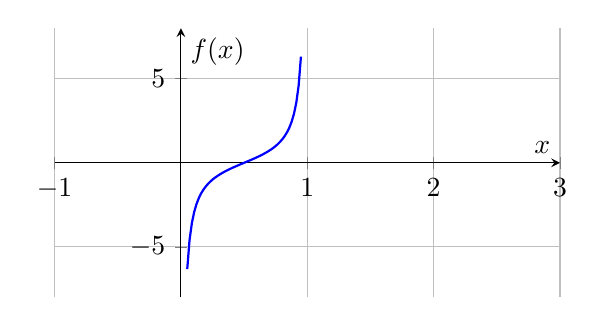
\begin{tikzpicture}
	\begin{axis}[
			axis lines = middle,
			xlabel = {\(x\)},
			ylabel = {\(f(x)\)},
			ymin=-8, ymax=8, % 设置 y 轴的范围
			xmin=-1, xmax=3, % 设置 x 轴的范围
			domain=0.05:0.95, % 设置函数的定义域
			samples=50, % 设置采样点数
			grid=both, % 显示网格
			width=8cm, % 设置图像的宽度
			height=5cm, % 设置图像的高度
		]
		\addplot [thick, blue] {tan(deg(pi*x - pi/2))}; % 绘制函数图像
	\end{axis}
\end{tikzpicture}

\end{document}
